\documentclass[runningheads]{llncs}

\usepackage{kotex}
\usepackage{graphicx}
\usepackage{placeins}
\usepackage{flafter}
\usepackage{booktabs}
\usepackage{multirow}
\usepackage{array}
\usepackage{amsmath,amssymb}
\usepackage{url}
\usepackage{microtype}
\emergencystretch=2em
\setlength{\textfloatsep}{8pt plus 2pt minus 2pt}
\setlength{\floatsep}{6pt plus 2pt minus 2pt}
\setlength{\intextsep}{6pt plus 2pt minus 2pt}

% ICISC 2026 익명 심사용 한국어 마스터 초안
% 최종 제출은 영어 LNCS 원고로 변환한다.
% 저자명/소속/사사/과제번호/식별 가능한 저장소 URL은 review 버전에서 제외한다.

\begin{document}

\title{이종 게임 MOD 패키지의 저작권 출처 판별을 위한 서버 기반 다중 출처 Provenance 복원 기법}
\titlerunning{게임 MOD 저작권 출처 판별을 위한 다중 출처 Provenance 복원}
\author{익명 저자}
\authorrunning{익명 저자}
\institute{익명 기관}
\maketitle

\begin{abstract}
게임 MOD 패키지는 Java 바이트코드, 구조화 리소스, 이미지 등 서로 다른 형태의 구성요소를 포함하며, 하나의 패키지가 여러 기존 MOD의 일부를 재조합하거나 분석 gallery에 등록되지 않은 출처의 콘텐츠를 포함할 수 있다. 저작권 출처 검토를 위해서는 하나의 패키지를 단일 출처로 가정하지 않고 구성요소별 기술적 원출처를 판별할 수 있어야 한다. 기존의 pairwise clone detection이나 단일 패키지 유사도만으로는 구성요소별 출처와 패키지 전체의 다중 부모 계보를 동시에 설명하기 어렵다.

본 연구는 저작권 출처 판별을 지원하기 위해, 이종 게임 MOD 패키지의 구성요소를 등록 부모 또는 개방집합 \texttt{UNKNOWN}으로 귀속하고 패키지 수준의 부모 집합을 복원하는 서버 기반 Hierarchical Multi-Parent Provenance Reconstruction 방법을 제안한다. 제안 방법은 CODE\_BINARY, STRUCTURED, IMAGE에서 path, project name, namespace와 같은 직접 식별 단서를 제외한 identity-neutral content evidence를 추출하고, 전역 후보 부모 검색, 제한된 parent-set 추론, 계층적 구성요소 할당을 수행한다. Dependency topology는 후보 집합 내부의 선택적 보정으로만 사용한다.

실제 공개 MOD의 current/historical release를 기반으로 120-project corpus와 540개 frozen query를 구축하였으며, 최종 TEST는 K1, K2, K3, mixed known/unknown, unknown-only 조건의 360개 query와 2,520개 component로 구성된다. 최종 방법은 component accuracy 0.805952, \texttt{UNKNOWN} F1 0.753786, parent-set F1 0.844233을 기록하였다. Hierarchical content-only reconstruction은 independent attribution 대비 parent-set exact match를 0.286111에서 0.413889로 향상시켰으며, graph refinement의 parent-set F1 증분은 +0.000688로 통계적으로 명확하지 않았다. FastAPI 기반 materialized end-to-end 분석은 p50 26.88 ms를 기록하였고, 전체 489개 component error 중 325개(66.46\%)가 retrieval 이후 component assignment 단계에서 발생하였다.

본 시스템은 저작권의 귀속이나 침해 여부를 자동 판정하지 않는다. 대신 업로드된 MOD 구성요소와 등록 참조 콘텐츠 사이의 기술적 provenance를 복원하여 콘텐츠 재사용 및 저작권 관련 출처 판별을 위한 인간의 검토에 기술적 증거를 제공한다.

\keywords{Copyright-Related Source Attribution \and Software Provenance \and Game MOD \and Multi-Parent Reconstruction \and Open-Set Attribution \and Software Reuse}
\end{abstract}

\section{서론}

게임 개발과 MOD 제작에서는 코드, 설정 데이터, 미디어 자산이 반복적으로 재사용된다. 게임 소프트웨어 공학의 실증 연구는 코드뿐 아니라 prefab과 같은 상위 수준 자산에서도 재사용이 이루어짐을 보여 준다 \cite{trasobares2025reuse}. 직접 복사나 재패키징은 package manager metadata에 남지 않을 수 있으므로, software supply-chain framework, secure-development 지침과 software bill of materials 표준은 검증 가능한 artifact provenance와 component inventory를 강조한다 \cite{torresarias2019intoto,nist2022ssdf,iso5962spdx}. 실제 supply-chain attack에 대한 실증 연구도 package 경계를 넘는 transformation evidence 보존의 필요성을 뒷받침한다 \cite{ohm2020backstabber}. 게임 MOD의 저작권 관련 출처 검토에서는 서로 다른 project에서 유래한 Java class, structured resource, image가 하나의 패키지에 함께 포함될 수 있고, 일부 출처는 server gallery에 존재하지 않을 수 있다. 따라서 기술적으로 필요한 것은 heterogeneous component의 개별 귀속, 여러 registered parent의 복원, 그리고 설명되지 않는 content의 open-set \texttt{UNKNOWN} 유지이다.

Clone detection과 software composition analysis는 code/library reuse 식별에 강하지만 일반적으로 clone pair나 library match를 출력한다 \cite{roy2008nicad,sajnani2016sourcerer,heinze2026stone}. Third-party library 식별은 packaged Java/Android와 native binary까지 분석 범위를 확장한다 \cite{backes2016libscout,bincofer2025}. Provenance 표준과 secure supply-chain 연구는 artifact의 derivation과 transformation을 모델링한다 \cite{w3c2013provdm,torresarias2019intoto}. 본 연구는 heterogeneous game MOD package에서 component-level registered-parent/\texttt{UNKNOWN} attribution과 package-level multi-parent reconstruction을 함께 수행하는 문제에 초점을 둔다.

이를 위해 Server-Side Hierarchical Multi-Parent Provenance Reconstruction을 제안한다. Path, project name, namespace를 제거한 identity-neutral CODE\_BINARY, STRUCTURED, IMAGE evidence를 추출하고, 전체 gallery에서 candidate parent를 검색한 뒤 bounded package-level parent set으로 component assignment를 제한한다. Dependency topology는 optional refinement로만 사용한다. 실제 공개 MOD 120개와 historical release에서 project-level calibration, registered TEST, held-out UNKNOWN split을 갖는 540개 frozen query를 구축하였다. 최종 360-query TEST에서 parent-set F1 0.844233을 기록했으며 external source baseline, FastAPI server, multi-UNKNOWN stress, retrieval scaling, failure localization도 평가하였다.

본 연구의 기여는 다음과 같다.
\begin{enumerate}
    \item heterogeneous MOD component와 package-level lineage의 기술적 출처 판별을 위한 open-set multi-parent formulation;
    \item retrieval, parent-set inference, component assignment, graph refinement를 분리한 hierarchical identity-neutral procedure;
    \item project-level split, held-out UNKNOWN, leakage control, exact provenance를 갖는 frozen real-MOD benchmark; 그리고
    \item analyst-facing source evidence를 대상으로 한 accuracy, uncertainty, ablation, NiCadCross, server latency, multi-UNKNOWN, Exact-versus-LSH scaling, failure localization의 frozen evaluation이다.
\end{enumerate}
시스템 출력은 technical provenance evidence이며 저작권 소유 또는 침해를 자동 판정하지 않는다.

\section{배경 및 관련 연구}

\subsection{코드 유사도, Clone Detection 및 Software Composition Analysis}
Code similarity는 text, token, AST, graph, learned representation을 사용하며 기존 비교 연구와 최근 systematic review는 benchmark, evaluation, language support의 지속적인 한계를 지적한다 \cite{roy2009comparison,zakeri2023slr}. NiCad는 source normalization 기반 near-miss clone 탐지 \cite{roy2008nicad}, SourcererCC는 token filtering/indexing 기반 large-scale detection \cite{sajnani2016sourcerer}, 최근 연구는 transformer clone detection과 interpretability를 결합한다 \cite{clonexformer2025}. Package/library 수준에서는 LibScout가 obfuscation에 강건한 Java/Android library를 탐지하고 \cite{backes2016libscout}, BinCoFer는 partial C/C++ binary TPL reuse를 다루며 \cite{bincofer2025}, 정식 심사를 거친 Android 연구는 obfuscation, versioning과 dependency-fusion 문제를 분석한다 \cite{androidtpl2025,libmd2025}. 이들은 reuse를 식별하지만 하나의 heterogeneous package에서 여러 project parent와 open-set unknown을 함께 복원하지는 않는다.

\subsection{게임 소프트웨어 재사용과 저작권 관련 출처 검토}
게임에서는 script, prefab, asset, scene-related resource가 함께 재사용될 수 있어 practical reuse unit이 단일 source file보다 넓다 \cite{trasobares2025reuse}. Software license audit 연구는 package declaration을 file-level artifact와 dependency relation에 대조해야 함을 보여 준다 \cite{german2010licensing}. 저작권 관련 검토에는 clone pair뿐 아니라 modality별 source 후보, mixed-source 관계와 gallery가 설명하지 못하는 component도 필요하다. 따라서 executable, structured, decoded-image evidence를 인간 검토용 기술 증거로 분리하며 소유권, 이용 허락, license status 또는 침해를 추론하지 않는다.

\subsection{Provenance, Lineage 및 Multi-Source Reconstruction}
일반 provenance 표준은 entity, activity, agent와 derivation을 구분하고 \cite{w3c2013provdm}, in-toto는 인증된 software supply-chain 단계를 기록하며 \cite{torresarias2019intoto}, ISO/IEC 5962는 SPDX component metadata를 표준화한다 \cite{iso5962spdx}. 이러한 artifact 및 metadata 수준 framework는 본 연구를 보완하지만 component-level multi-parent reconstruction 자체를 수행하지는 않는다. 본 연구의 novelty는 ``heterogeneous provenance'' 또는 ``multi-parent''라는 용어 자체가 아니라 component-level registered-parent/\texttt{UNKNOWN} attribution, package-level reconstruction, frozen real-MOD benchmark, server-side evaluation의 구체적 결합에 있다.

\section{시스템 및 문제 모델}

\subsection{서버 사용 시나리오}

분석 서버는 사전에 등록된 reference MOD를 유지한다. 등록 단계에서는 package를 component로 분해하고 identity-neutral evidence로 parent별 gallery를 구축한다. Online analysis는 업로드 archive에 같은 extractor를 적용하여 reconstructed parent set, component label과 \texttt{UNKNOWN} 판정을 반환한다. Report는 인간의 registered-candidate 비교를 돕지만 법적 지위를 확정하거나 gallery 부재를 독창성으로 간주하지 않는다.

\begin{figure}[!htbp]
    \centering
    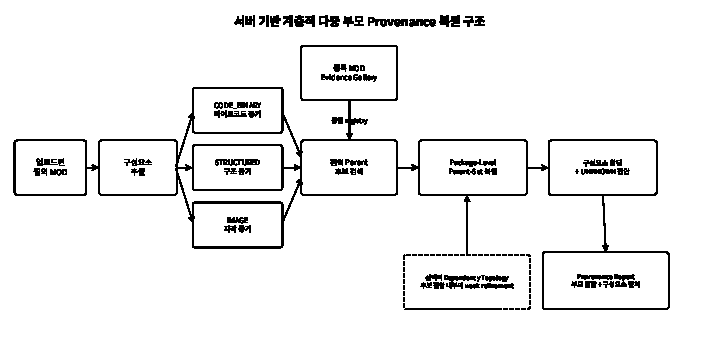
\includegraphics[width=0.90\linewidth]{figures/system_overview_ko.pdf}
    \caption{제안 시스템의 online provenance reconstruction 흐름. CODE, STRUCTURED, IMAGE의 identity-neutral content evidence가 핵심이며 dependency topology는 후보 집합 내부의 선택적 보정으로만 사용한다.}
    \label{fig:system}
\end{figure}
\FloatBarrier



\subsection{Multi-Parent Open-Set 정의}

등록 reference gallery를
\[
\mathcal{G}=\{G_1,\ldots,G_N\}
\]
로 정의한다. Query MOD는 component set과 선택적 dependency edge로 이루어진
\[
G_q=(V_q,E_q)
\]
로 표현한다. 각 component \(v\in V_q\)는
\[
m(v)\in\{\textsc{Code},\textsc{Structured},\textsc{Image}\}
\]
의 modality를 가지며, provenance label은
\[
y_v\in\{1,\ldots,N,\textsc{Unknown}\}
\]
이다. Package-level registered parent set은
\[
P_q=\{p\mid \exists v\in V_q,\;y_v=p,\;p\neq\textsc{Unknown}\}
\]
로 정의한다. 시스템은 component label \(\hat y_v\)뿐 아니라 \(\hat P_q\)와 registered-parent count \(\hat K=|\hat P_q|\)를 함께 출력한다.

본 연구에서 \texttt{UNKNOWN}은 ``새로운 저작물'' 또는 ``독창적인 콘텐츠''를 의미하지 않는다. 단지 현재 server-side registered gallery로 설명할 수 없는 출처를 의미한다. 서로 다른 unknown source가 여러 개 존재하더라도 primary model은 하나의 collapsed \texttt{UNKNOWN} label만 제공한다.

\subsection{분석 가정과 Hard Evaluation Track}

본 연구는 공격자가 특정 adversarial transformation을 수행한다고 가정하지 않는다. 대신 provenance model이 path나 naming convention 같은 쉬운 identity cue에 의존하지 않도록 hard evaluation track을 정의한다. Final attribution method에는 original relative path, basename, MOD namespace, source project identity, source SHA-256, ground-truth label을 입력하지 않는다. Java code에서도 method/class name, descriptor, string constant, constant-pool operand와 같은 직접 식별 정보를 representation에서 제외한다.

이 설계는 ``이름이 같아서 같은 MOD라고 맞히는'' trivial solution을 방지하고, 실제 content structure와 behavior-related pattern이 provenance evidence로 작동하도록 하기 위한 것이다. 다만 이는 모든 형태의 obfuscation이나 semantics-preserving transformation을 완전히 방어한다는 의미는 아니다.

\subsection{구조적 목적함수}

전체 decision은 다음 structured objective로 개념화할 수 있다.
\[
\hat{\mathbf y}=\arg\min_{\mathbf y}
\left[
\sum_{v\in V_q}\phi_v(y_v)
+\gamma\Omega(\mathbf y)
+\beta\sum_{(u,v)\in E_q}\psi_{uv}(y_u,y_v)
\right],
\]
여기서 \(\phi_v\)는 heterogeneous content evidence에 기반한 component-parent assignment cost이고, \(\Omega\)는 불필요한 parent proliferation을 억제하는 package-level penalty, \(\psi_{uv}\)는 dependency consistency를 표현하는 선택적 항이다. 실제 구현에서는 전체 gallery를 직접 조합 탐색하지 않고 candidate retrieval과 bounded parent-set search로 분해한다.

\section{제안 방법}

\subsection{전체 처리 흐름}

제안 방법은 (1) component extraction, (2) modality별 identity-neutral evidence extraction, (3) component-to-parent distance 계산, (4) package-level candidate retrieval, (5) bounded parent-set reconstruction, (6) component assignment 및 \texttt{UNKNOWN} rejection, (7) 선택적 dependency refinement의 순서로 수행된다. 핵심 설계는 component evidence와 package-level decision을 분리하는 것이다. Independent classifier에서는 한두 개의 noisy component가 새로운 false parent를 추가할 수 있지만, hierarchy는 query 전체 evidence를 이용해 작은 parent set을 먼저 선택함으로써 이를 억제한다.

\subsection{CODE\_BINARY Evidence}

Java class file은 method-level opcode sequence를 parsing한다. Identity-neutral CODE representation은 Charikar가 제안한 compact similarity sketch 원리에 기반한 세 종류의 128-bit SimHash를 사용한다 \cite{charikar2002simhash}.

첫째, opcode 3-gram representation은 operand나 constant value를 사용하지 않고 opcode sequence 자체의 local pattern만 보존한다. 둘째, structural representation은 method length, max stack, max locals, access flag, opcode category count, class-level method/field/instruction count를 log-bucket으로 요약한다. 셋째, context representation은 arithmetic, branch, load/store, invoke 등 opcode category의 3-gram을 사용한다. 이 방식은 class name, method name, descriptor, string literal과 같은 직접 identity information을 사용하지 않으면서 control/operation structure를 일정 수준 보존한다.

\subsection{STRUCTURED Evidence}

JSON과 유사한 structured resource에서는 literal identifier 자체보다 구조와 value shape를 보존한다. 이는 canonical JSON representation이 강조하는 재현 가능성에 기반하되 \cite{rundgren2020jcs}, benchmark-specific encoding에서는 identity-neutral structural category만 유지한다. Key/value traversal 과정에서 object/array depth, key category, numeric/string/boolean/null pattern, sequence structure를 token으로 변환하고 128-bit SimHash로 요약한다. Resource identifier가 \texttt{namespace:path} 형태인 경우 \texttt{minecraft}와 같은 external namespace는 category로 유지하지만 MOD-specific namespace literal은 노출하지 않는다. 긴 hex, URL, qualified identifier 역시 literal을 그대로 사용하지 않고 shape category로 변환한다.

빈 JSON object와 같이 다수 project에서 반복되며 provenance information이 거의 없는 trivial structured component는 benchmark preprocessing 단계에서 제거한다.

\subsection{IMAGE Evidence}

IMAGE는 file name이나 path를 사용하지 않고 decoded pixel만 분석한다. Grayscale image에서 64-bit aHash, dHash, pHash를 추출하고, luminance distribution을 16-bin normalized histogram으로 계산한다. Perceptual image hashing은 시각적으로 중요하지 않은 변환에 안정적으로 설계되므로 \cite{monga2006perceptual}, 이렇게 생성한 evidence는 lossless re-encoding처럼 byte-level SHA가 달라져도 시각 content가 유지되는 경우를 처리할 수 있다. Final benchmark의 IMAGE payload는 lossless PNG re-encoding을 사용하며 pixel equality를 검증하였다.

\subsection{Component-to-Parent Cost}

각 query component는 동일 modality의 gallery component와 비교된다. Binary signature 간에는 normalized Hamming distance를 사용하고 image histogram에는 normalized \(L_1\) distance를 사용한다. Parent \(p\)에 대한 component distance \(d(v,p)\)는 해당 parent가 보유한 같은 modality gallery component 중 가장 가까운 evidence를 기반으로 계산한다.

Representation별 거리를 normalize한 뒤 strongest visible parent 대비 상대적인 regret를 함께 사용한다. Frozen component cost는 개념적으로
\[
c(v,p)=\alpha\,\tilde d(v,p)+(1-\alpha)\,\tilde r(v,p)
\]
로 표현하며 \(\alpha=0.75\), regret weight는 0.25이다. Modality별 open-set threshold는 calibration split에서만 결정한다.

\subsection{Global Candidate Retrieval}

전체 registered parent를 package reconstruction에서 직접 조합하면 후보 조합 수가 빠르게 증가한다. 따라서 먼저 query-level retrieval score를 계산하여 탐색 공간을 제한한다. Query $q$에서 parent $p$에 대한 retrieval score는 component cost 가운데 가장 작은 $L=3$개를 집계한 값으로 정의한다. 직관적으로는 한두 개의 강한 provenance evidence가 존재하는 parent를 우선 남기되, 단일 우연 match 하나만으로 ranking이 결정되지 않도록 하는 방식이다.

\[
R_q(p)=\frac{1}{L}\sum_{i=1}^{L} c_{(i)}(p),\qquad L=3,
\]
여기서 $c_{(i)}(p)$는 parent $p$에 대한 query component cost를 오름차순으로 정렬했을 때 $i$번째 값이다. $R_q(p)$가 작은 상위 $M=10$개의 parent를 candidate pool $C_q$로 유지한다. TEST에서 mean registered-parent recall은 0.974444이며 applicable query의 0.943333에서 모든 true registered parent가 candidate pool에 포함되었다.

\subsection{Hierarchical Parent-Set Reconstruction}

Candidate pool $C_q$에 대해 $|S|\le K_{\max}=3$인 parent subset $S\subseteq C_q$를 탐색한다. 주어진 $S$에서 component $v$는 $S\cup\{\textsc{Unknown}\}$ 중 가장 낮은 frozen assignment cost를 갖는 label을 선택한다. Package-level objective는 component fit와 parent 수 penalty를 결합한다.

\[
J_q(S)=\sum_{v\in V_q}\min_{y\in S\cup\{\textsc{Unknown}\}} c(v,y)+\lambda |S|,
\]
\[
\hat S_q=\arg\min_{S\subseteq C_q,\ |S|\le K_{\max}} J_q(S),\qquad \lambda=0.5.
\]

이 계층은 component-level local optimum이 query마다 지나치게 많은 parent를 생성하는 현상을 억제한다. Graph를 사용하는 final variant에서는 selected subset 내부의 boundary-consistency term을 작은 weight로 추가하지만, content-only variant의 objective와 candidate pool은 동일하다.

\begin{table}[!htbp]
\centering
\caption{Hierarchical Multi-Parent Provenance Reconstruction의 구현 절차.}
\label{tab:algorithm}
\scriptsize
\begin{tabular}{p{0.08\linewidth}p{0.84\linewidth}}
\toprule
단계 & 처리\\
\midrule
1 & Query package에서 CODE\_BINARY, STRUCTURED, IMAGE component를 추출한다.\\
2 & 각 component에서 identity-neutral evidence를 계산한다.\\
3 & 동일 modality gallery와 비교하여 component-parent cost를 계산한다.\\
4 & Query-level evidence를 aggregate하여 상위 \(M=10\) registered parent를 검색한다.\\
5 & Candidate pool에서 \(|S|\le3\)인 parent subset을 평가한다.\\
6 & 각 subset에 대해 registered parent 또는 \texttt{UNKNOWN}으로 component를 할당한다.\\
7 & Parent-count penalty와 선택적 graph term을 포함한 package objective가 최소인 subset을 선택한다.\\
8 & Final parent set, \(\hat K\), component labels, uncertainty-related evidence를 provenance report로 반환한다.\\
\bottomrule
\end{tabular}
\end{table}

\subsection{UNKNOWN 처리}

Open-set threshold는 modality별 calibration에서 결정하고 TEST 이전에 고정한다. Frozen threshold는 CODE 0.1302083284, STRUCTURED 0.03125, IMAGE 0이다. IMAGE threshold가 0이라는 것은 해당 frozen representation/calibration에서 registered-parent match에 매우 보수적인 exact-nearest condition이 선택되었음을 의미하며, 다른 데이터셋에 보편적인 threshold라는 의미가 아니다.

Primary TEST에서는 query당 최대 하나의 held-out unknown source를 사용한다. 그러나 후속 robustness 분석에서는 두 개 또는 세 개의 distinct held-out donor를 하나의 query에 포함시켜 collapsed \texttt{UNKNOWN} rejection의 안정성을 별도로 평가한다.

\subsection{선택적 Dependency Refinement}

Dependency graph는 주로 Java class reference로 구성되며 non-class edge는 sparse하다. 따라서 본 연구는 이를 ``fully heterogeneous provenance graph''로 주장하지 않는다. Graph evidence는 candidate pool 내부의 selected parent assignment를 약하게 보정하는 역할만 수행하며 frozen weight는 \(\beta=0.1\)이다. Connected stress track은 서로 다른 parent의 code component 사이에 deterministic bridge가 존재하는 상황에서 구조적 grouping이 얼마나 취약한지를 보기 위한 controlled stress이다. 이러한 실험 결과를 반영하여 graph는 최종 논문의 중심 contribution이 아니라 optional refinement로 위치시킨다.


\section{벤치마크 구축 및 실험 설계}

\subsection{실제 MOD Corpus와 Historical Release}

최종 corpus는 120개의 실제 공개 MOD project로 구성하였다. 역할 기준으로 90개는 target project, 30개는 background project이다. 각 project에 대해 current release와 가능한 historical release를 수집하고 component registry를 생성하였다. 필터 적용 전 current registry에는 60,257개, historical registry에는 178,162개의 component가 존재하였다.

Empty JSON object처럼 provenance signal이 거의 없는 trivial structured component는 사전에 제거하였다. 필터 후 registry는 current 56,035개, historical 165,496개 component로 구성되었고, current corpus의 cross-project exact-SHA duplicate는 5개 group(48개 component)으로 제한적이었다. 이를 통해 반복되는 trivial resource가 benchmark를 지배하는지 사전 점검하였다.

\subsection{Identity Leakage Audit}

Historical target component 124,470개를 대상으로 current release와의 identity overlap을 조사하였다. 자신의 current release에 exact SHA-256이 존재하지 않는 historical component를 hard-masked candidate로 정의하였으며 31,279개가 해당 조건을 만족하였다. 이 중 같은 full relative path도 current에 존재하지 않는 stricter subset은 6,429개였다.

TEST\_KNOWN historical component 전체에서는 own exact-SHA survival rate가 0.677471인 반면 same-path rate는 0.919728이었다. 이는 path/name을 그대로 사용하면 content transformation보다 훨씬 쉬운 identity cue가 될 수 있음을 보여준다. 따라서 final method에서는 path, basename, namespace, source project identity를 사용하지 않는다.

\begin{figure}[!htbp]
    \centering
    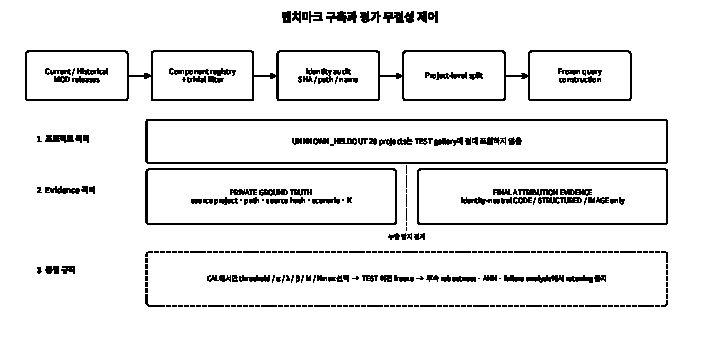
\includegraphics[width=0.88\linewidth]{figures/leakage_freeze_ko.pdf}
    \caption{Benchmark construction과 evaluation-integrity control. Project-level open-set 격리, private ground truth와 final attribution evidence의 분리, CAL-only tuning과 TEST 이전 freeze를 함께 적용한다.}
    \label{fig:leakage}
\end{figure}
\FloatBarrier

\subsection{Project Split과 Open-Set 분리}

Project split은 component-level split보다 먼저 고정하였다. 이는 동일 project의 highly similar release가 calibration과 TEST 양쪽에 동시에 노출되는 것을 방지하기 위한 것이다.

\begin{table}[!htbp]
\centering
\caption{동결된 project-level split.}
\label{tab:split}
\scriptsize
\begin{tabular}{lrr}
\toprule
Split & Projects & 역할\\
\midrule
CAL\_KNOWN & 25 & calibration용 registered target\\
TEST\_KNOWN & 45 & final TEST용 registered target\\
UNKNOWN\_HELDOUT & 20 & gallery에 없는 open-set source\\
CAL\_BACKGROUND & 15 & calibration gallery background\\
TEST\_BACKGROUND & 15 & TEST gallery background\\
\bottomrule
\end{tabular}
\end{table}

Calibration gallery는 40개 project, TEST gallery는 60개 project로 구성된다. UNKNOWN\_HELDOUT 20개 project는 TEST gallery에 단 하나도 포함되지 않는다. Hard masking과 fixed modality composition 조건까지 통과하여 실제 query donor로 사용 가능한 project pool은 CAL\_KNOWN 19개, TEST\_KNOWN 33개, UNKNOWN\_HELDOUT 15개였다.

\subsection{자동 Query 생성과 Ground Truth}

Final benchmark는 수작업으로 ``어떤 파일이 어느 MOD에서 왔는지'' label을 붙이지 않는다. Historical component registry와 private source manifest를 이용하여 donor project와 source component를 자동 선택하고, query manifest에 exact component origin을 기록한다. 이후 source identity가 드러나지 않는 public/materialized payload만 evaluation pipeline에 제공한다.

총 540개 query를 생성하였다. Calibration은 180개, TEST는 360개이며 각 query는 정확히 7개 component로 구성된다.
\[
5\ \textsc{Code}
+
1\ \textsc{Structured}
+
1\ \textsc{Image}.
\]
따라서 전체 materialized payload는 3,780개이다. 540개 IMAGE는 모두 lossless PNG로 다시 encoding하였고, 모든 image에 대해 decoded pixel equality를 확인하였다. Source hash verification 역시 3,780/3,780 payload에서 통과하였다.


TEST는 Table~\ref{tab:scenario}의 여섯 scenario를 각각 60개씩 포함한다.

\begin{table}[!htbp]
\centering
\caption{Frozen TEST의 scenario 구성.}
\label{tab:scenario}
\scriptsize
\begin{tabular}{lrrr}
\toprule
Scenario & Queries & Registered parents & Unknown sources\\
\midrule
TEST\_KNOWN\_K1 & 60 & 1 & 0\\
TEST\_KNOWN\_K2 & 60 & 2 & 0\\
TEST\_KNOWN\_K3 & 60 & 3 & 0\\
TEST\_MIXED\_1K1U & 60 & 1 & 1\\
TEST\_MIXED\_2K1U & 60 & 2 & 1\\
TEST\_UNKNOWN\_K1 & 60 & 0 & 1\\
\bottomrule
\end{tabular}
\end{table}

실제 total-source count 기준 K=1, K=2, K=3 query가 각각 120개로 균형을 이룬다. Public manifest에는 K, scenario, source identity, path, source hash를 노출하지 않는다.

\subsection{Graph Track}

선택된 5개 CODE component에 대해 historical CLASS\_REF edge를 이용한 NATURAL graph를 보존하였다. 별도의 CONNECTED\_STRESS track은 parent label이나 K를 사용하지 않고 필요한 최소 deterministic bridge를 추가하여 5개 code node를 연결한다. 이는 실제 자연 graph라고 주장하기 위한 것이 아니라, cross-parent bridge가 존재하는 경우 graph-based grouping이 얼마나 취약할 수 있는지를 보는 controlled structural stress이다.

\subsection{Calibration과 Freeze Discipline}

모든 threshold 및 reconstruction hyperparameter는 calibration에서만 결정하였고 TEST prediction을 확인한 후 변경하지 않았다.

Frozen configuration은 CODE threshold 0.1302083283662796, STRUCTURED 0.03125, IMAGE 0, content weight $\alpha=0.75$, regret weight 0.25, parent penalty $\lambda=0.5$, candidate $M=10$, graph weight $\beta=0.1$, boundary Top-$R=3$, $K_{\max}=3$이다. 후속 robustness, scalability, failure-analysis는 이 설정을 retune하지 않는다.



\subsection{통계 분석 및 재현성 Protocol}

Primary uncertainty는 7개 component를 하나의 query cluster로 유지하는 scenario-stratified bootstrap 10,000회로 계산하였다. Graph와 content-only 비교는 동일 query에 대한 paired bootstrap delta를 사용하였고, source project 반복의 영향을 확인하기 위해 source-anchor cluster bootstrap과 leave-one-source-project-out sensitivity를 추가 수행하였다. Parameter는 calibration split에서만 선택하였으며 TEST는 tuning에 사용하지 않았다.

Materialized TEST 2,520개 component를 raw payload에서 다시 추출했을 때 payload SHA-256이 모두 일치했고, 40,320개 evidence field 비교에서도 mismatch가 없었다. Query evidence table에는 source path, project ID, ground-truth label, scenario, K, source hash를 포함하지 않으며 UNKNOWN\_HELDOUT project가 gallery에 존재하지 않음을 programmatically 검사하였다.

\subsection{실험 환경}

Primary accuracy 실험과 server benchmark는 같은 conceptual pipeline을 사용하지만 목적이 다르므로 성능 수치를 혼합하지 않는다. Server benchmark의 host와 protocol은 Table~\ref{tab:environment}과 같다.

\begin{table}[!htbp]
\centering
\caption{Server-side benchmark 환경 및 protocol.}
\label{tab:environment}
\scriptsize
\begin{tabular}{p{4.1cm}p{7.1cm}}
\toprule
항목 & 설정\\
\midrule
Host OS & Windows 10, build 26200\\
Python & 3.10.6\\
CPU & 20 physical / 28 logical cores\\
Server & FastAPI / Uvicorn, single process\\
TEST gallery & 60 projects, 26,329 components\\
Concurrency & 1, 4, 8, 16, 32\\
Requests & 각 concurrency당 200 requests\\
Warm-up & 20 requests\\
Random seed & 20260813\\
Input & local materialized query ZIP; network upload time 제외\\
\bottomrule
\end{tabular}
\end{table}

External source baseline은 WSL Linux 환경에서 Open-NiCad/NiCadCross를 사용하였다. StoneDetector는 공식 구현의 modern Java bytecode/toolchain compatibility를 audit한 뒤 성능 baseline으로 과도하게 해석하지 않았다.

\subsection{평가 지표와 Research Questions}

Component level에서는 accuracy와 \texttt{UNKNOWN} precision/recall/F1, package level에서는 parent-set precision/recall/F1, exact match, K accuracy와 K MAE, retrieval level에서는 registered-parent recall을 측정한다. 연구 질문은 \textbf{RQ1} 저작권 관련 출처 복원 정확도, \textbf{RQ2} hierarchy/graph 기여, \textbf{RQ3} 호환 external clone baseline 비교, \textbf{RQ4} frozen decision을 재현하는 server 성능, \textbf{RQ5} multi-UNKNOWN/approximate retrieval 강건성, \textbf{RQ6} 잔여 error 발생 단계이다.

\section{실험 결과}

\subsection{RQ1: Frozen TEST의 주요 성능}
\begin{table}[!htbp]
\centering
\caption{Frozen primary TEST의 최종 성능.}
\label{tab:mainresult}
\scriptsize
\begin{tabular}{lr}
\toprule
Metric & Score\\
\midrule
Component Accuracy & 0.805952\\
UNKNOWN Precision & 0.652427\\
UNKNOWN Recall & 0.892430\\
UNKNOWN F1 & 0.753786\\
Parent-Set F1 & 0.844233\\
Exact Parent-Set Match & 0.419444\\
K Accuracy & 0.486111\\
K MAE & 0.527778\\
Candidate mean registered-parent recall & 0.974444\\
All true registered parents present & 0.943333\\
\bottomrule
\end{tabular}
\end{table}
최종 방법은 component accuracy 0.805952, \texttt{UNKNOWN} F1 0.753786, parent-set F1 0.844233을 기록하였다. Exact match 0.419444와 K accuracy 0.486111은 parent identity가 일부 복원되어도 정확한 source-count 추론이 어렵다는 점을 보여준다.

\subsection{Scenario별 성능}
\begin{table}[!htbp]
\centering
\caption{Frozen TEST의 scenario별 final result. 각 scenario는 60 query이다.}
\label{tab:scenarioresult}
\scriptsize
\begin{tabular}{lccccc}
\toprule
Scenario & Comp. Acc. & Parent F1 & Exact & K Acc. & UNK F1\\
\midrule
Known K1 & 0.757143 & 0.750000 & 0.283333 & 0.283333 & --\\
Known K2 & 0.809524 & 0.843333 & 0.316667 & 0.383333 & --\\
Known K3 & 0.745238 & 0.787937 & 0.100000 & 0.333333 & --\\
Mixed 1K1U & 0.828571 & 0.930556 & 0.700000 & 0.716667 & 0.847059\\
Mixed 2K1U & 0.797619 & 0.917460 & 0.600000 & 0.683333 & 0.739550\\
UNKNOWN-only & 0.897619 & 0.836111 & 0.516667 & 0.516667 & 0.946048\\
\bottomrule
\end{tabular}
\end{table}
Known K3의 exact match는 0.100000으로 가장 낮아 세 registered parent를 모두 동시에 복원하는 난도를 보여준다. Mixed scenario의 높은 parent-set F1은 source share가 다르고 unseen source를 하나의 \texttt{UNKNOWN}으로 collapse하기 때문에 causal result가 아닌 descriptive result로 해석한다.

\subsection{Modality별 성능}
\begin{table}[!htbp]
\centering
\caption{Frozen TEST의 modality별 final component result.}
\label{tab:modality}
\scriptsize
\begin{tabular}{lrrrr}
\toprule
Modality & Components & Comp. Acc. & UNK Recall & UNK F1\\
\midrule
CODE\_BINARY & 1,800 & 0.810000 & 0.893773 & 0.766091\\
IMAGE & 360 & 0.972222 & 0.911765 & 0.948980\\
STRUCTURED & 360 & 0.619444 & 0.866667 & 0.581470\\
\bottomrule
\end{tabular}
\end{table}
IMAGE가 가장 안정적이고 CODE\_BINARY가 중간, STRUCTURED가 가장 어렵다. Identifier 제거 뒤 유사한 structural shape가 반복되므로 structured-resource evidence와 modality-specific calibration 개선이 필요하다.

\subsection{불확실성: Query Bootstrap과 Source-Project Sensitivity}
Scenario-stratified query bootstrap 10,000회에서 95\% interval은 component accuracy [0.787698, 0.823810], parent-set F1 [0.829101, 0.859114], exact match [0.372222, 0.466667], K accuracy [0.436111, 0.533333], \texttt{UNKNOWN} F1 [0.732551, 0.774445]이다. Source-anchor bootstrap의 parent-set F1은 [0.820531, 0.867090]이며 leave-one-source-project-out 최대 변화는 parent-set F1 0.005836, component accuracy 0.011392로 작았다.

\subsection{RQ2: Hierarchical Reconstruction의 효과}
\begin{table}[!htbp]
\centering
\caption{Independent attribution, hierarchical content, final graph의 비교.}
\label{tab:ablation}
\scriptsize
\begin{tabular}{lccccc}
\toprule
Method & Comp. Acc. & UNK F1 & Parent F1 & Exact & K Acc.\\
\midrule
Independent & 0.775794 & 0.741806 & 0.797412 & 0.286111 & 0.325000\\
Hierarchical content & 0.807143 & 0.752386 & 0.843545 & 0.413889 & 0.480556\\
Final + graph & 0.805952 & 0.753786 & 0.844233 & 0.419444 & 0.486111\\
Oracle-K content & 0.825794 & 0.790948 & 0.872976 & 0.558333 & 0.627778\\
\bottomrule
\end{tabular}
\end{table}
Hierarchical content-only는 independent attribution 대비 component accuracy +0.031349, parent-set F1 +0.046133, exact match +0.127778, K accuracy +0.155556을 개선한다. Graph의 parent-set F1 증분은 +0.000688이고 paired-bootstrap 95\% interval [-0.001693, 0.003466]은 0을 포함한다. Oracle-K exact match 0.558333은 K inference가 주요 residual bottleneck임을 보여준다.

\subsection{RQ3: External Source-Level Baseline}
NiCadCross는 source-resolvable TEST CODE 1,169개에서 평가하며 gallery CODE는 3,275/10,448개가 source-resolvable하다. Functions/Java/default blind-renaming, threshold 0.30에서 query parse failure 10개, gallery failure 19개, clone pair 2,199개, matched class 505개가 생성되었다.
\begin{table}[!htbp]
\centering
\caption{동일한 1,169개 source-resolvable component에서 NiCadCross와 제안 방법 비교.}
\label{tab:nicad}
\scriptsize
\begin{tabular}{lccccc}
\toprule
Method & Comp. Acc. & UNK F1 & Parent F1 & Exact & K Acc.\\
\midrule
NiCadCross & 0.710009 & 0.678673 & 0.815468 & 0.725490 & 0.588235\\
Proposed & 0.840890 & 0.794016 & 0.867429 & 0.787582 & 0.771242\\
\bottomrule
\end{tabular}
\end{table}
Paired query-bootstrap interval은 component accuracy [0.096187, 0.166524], \texttt{UNKNOWN} F1 [0.079256, 0.154288], K accuracy [0.114379, 0.251634]에서 제안 방법에 유리하지만 exact-match delta는 0을 포함한다. NiCad는 reconstructed Java source를 받으므로 same-subset comparison으로 해석하고 universal superiority를 주장하지 않는다. StoneDetector는 modern bytecode/toolchain 문제로 compatibility audit으로만 사용한다.

\subsection{RQ4: 실제 Server-Side Evaluation}
\subsubsection{Offline-Server Correctness.}
Single-process FastAPI/Uvicorn server는 360/360 frozen TEST query에서 candidate top-10, selected subset, K, 2,520개 assignment를 모두 동일하게 재현하였다.

\subsubsection{Materialized End-to-End Latency.}
Benchmark에는 archive/manifest parsing, payload read, raw evidence extraction, 60-project gallery search, reconstruction, graph refinement, response construction을 포함하고 network upload는 제외한다.
\begin{table}[!htbp]
\centering
\caption{Materialized package 단일 요청의 p50 latency breakdown.}
\label{tab:latency}
\scriptsize
\begin{tabular}{lr}
\toprule
Stage & p50 latency\\
\midrule
Archive open + manifest & 0.334 ms\\
Payload read & 0.232 ms\\
Identity-neutral extraction & 14.440 ms\\
60-project gallery search & 10.685 ms\\
Reconstruction & 1.086 ms\\
Total server processing & 26.880 ms\\
\bottomrule
\end{tabular}
\end{table}
Concurrency 1의 total p50은 26.880 ms이며 extraction 14.440 ms와 search 10.685 ms가 reconstruction 1.086 ms보다 크다.

\subsubsection{Concurrency and Throughput.}
Concurrency 1, 4, 8, 16, 32에서 각각 200 request를 측정한 1,000 request가 모두 성공하였다. Throughput은 24.72, 37.60, 38.00, 38.71, 37.16 req/s로 concurrency 16에서 peak를 보인 뒤 single-process contention의 영향을 받는다.

\subsubsection{Real-Project Gallery Scaling.}
Real gallery를 20에서 100 project로 늘리면 component는 16,282에서 48,376(2.97$\times$), search p50은 4.353에서 21.457 ms(4.93$\times$), reconstruction p50은 0.680에서 1.423 ms로 증가한다. 따라서 scale-up의 주된 target은 gallery search이다.

\subsection{RQ5: Multi-UNKNOWN 강건성과 Approximate Retrieval}
\subsubsection{Controlled Multi-UNKNOWN Stress.}
두세 개 distinct held-out donor를 포함하는 post-freeze 180-query stress test는 component accuracy 0.841270, \texttt{UNKNOWN} F1 0.887991, collapsed parent-set F1 0.883968, exact match 0.600000, collapsed K accuracy 0.633333을 기록한다. Registered parent를 포함한 120 query의 precision/recall/F1은 0.815278/0.912500/0.840556, exact match는 0.625000이다. Rejection은 안정적이지만 unknown identity와 multiplicity 자체를 복원하지는 않는다.

\subsubsection{Exact-versus-LSH Retrieval.}
BALANCED와 HIGH\_RECALL은 Exact content-only prediction을 모두 재현하고 FAST는 360 query 중 1개, 2,520 component 중 1개만 변경한다(component accuracy 0.806746 vs. 0.807143, parent-set F1 0.842804 vs. 0.843545).
\begin{figure}[!htbp]
    \centering
    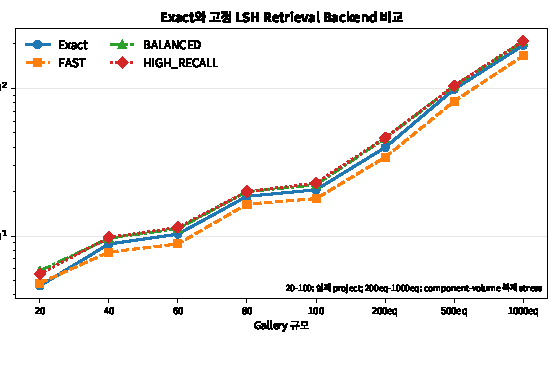
\includegraphics[width=0.80\linewidth]{figures/phase12_scalability_ko.pdf}
    \caption{Exact와 세 LSH configuration의 retrieval p50. 20--100은 실제 registered-project scale이고 200eq--1000eq는 100개 real parent의 component array를 복제한 computational volume stress이다.}
    \label{fig:lsh}
\end{figure}
60-project runtime sample에서 FAST는 p50을 10.315에서 8.848 ms로 낮춰 1.166$\times$ speedup을 보였지만 fidelity-preserving LSH는 20--100 real project에서 Exact보다 빠르지 않았다.

\subsection{RQ6: Post-Freeze Failure Localization}
2,520개 component 중 489개가 error이며 358 known-to-\texttt{UNKNOWN}, 81 \texttt{UNKNOWN}-to-known, 50 wrong-known-parent transition으로 구성된다.
\begin{figure}[!htbp]
    \centering
    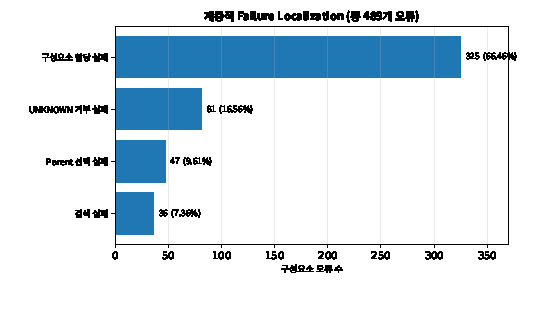
\includegraphics[width=0.70\linewidth]{figures/phase13_failure_breakdown_ko.pdf}
    \caption{Frozen TEST의 489개 component error에 대한 hierarchical failure localization.}
    \label{fig:failure}
\end{figure}
Component Assignment Miss가 325개로 가장 많고 Retrieval Miss는 36개이다. Query-level parent-set failure 209개는 reconstruction-limited 192개와 retrieval-limited 17개로 나뉜다. TEST\_KNOWN\_K1의 102개 error는 모두 assignment failure이고 K3에서는 retrieval miss 21개와 parent-selection miss 19개가 추가된다. 따라서 candidate recall만 높이기보다 assignment/\texttt{UNKNOWN} calibration과 K inference 개선이 우선이다.

\section{논의}
Ablation에서 핵심 개선은 graph가 아니라 hierarchy이다. Content-only reconstruction은 independent attribution 대비 parent-set F1, exact match, K accuracy를 크게 개선하지만 graph 증분은 statistically inconclusive하다. Failure localization에서 489개 error 중 325개가 true parent가 retrieval과 package-level selection을 통과한 뒤 발생했고 Oracle-K는 exact match를 0.413889에서 0.558333으로 높였다. 따라서 assignment calibration과 source-count inference가 주요 잔여 병목이다. Modality 난도도 IMAGE 0.972222, STRUCTURED 0.619444로 차이가 크며, runtime은 reconstruction보다 extraction과 gallery search가 지배한다.

저작권 관련 검토에서 이 시스템은 registered candidate를 좁히고 attribution을 국소화하며 unsupported content를 표시하는 triage/traceability layer이다. Score는 저자성, 소유권, 복제, 이용 허락, license 준수 또는 침해를 확정하지 않으며, \texttt{UNKNOWN}은 gallery evidence 부족만 뜻한다. 따라서 component와 reference에 대한 인간 검토가 필요하다.

\section{한계 및 타당성 위협}
Controlled recomposition은 exact technical donor label을 제공하지만 실제 refactoring, partial edit, image transformation, resource merge 전체를 재현하지 않는다. Benchmark는 법적 판단이 끝난 저작권 사건 corpus가 아니므로 본 지표는 provenance reconstruction을 측정하며 법적 저작권 판정의 정확도를 뜻하지 않는다. Identity leakage를 제거하고 re-extraction mismatch가 없음을 확인하였다. External validity는 120-project Java-centric corpus에 제한되고 200eq--1000eq는 독립 real project가 아닌 computational-volume stress이다. Graph delta는 유의하지 않으며 NiCadCross는 source-resolvable subset, StoneDetector는 compatibility audit으로만 해석한다. Model은 하나의 collapsed \texttt{UNKNOWN}만 제공하고 graph는 주로 Java class-reference backbone이며, latency는 특정 host에서 network upload를 제외해 측정했다. Post-freeze 분석은 primary TEST를 retune하지 않는다.

\section{결론}
본 연구는 heterogeneous game MOD package의 저작권 관련 출처 판별을 위한 server-side Hierarchical Multi-Parent Provenance Reconstruction을 제안하였다. 120개 real project와 historical release로 540개 frozen query와 3,780개 materialized component를 구축했고 360-query TEST에서 component accuracy 0.805952, \texttt{UNKNOWN} F1 0.753786, parent-set F1 0.844233을 얻었다. 핵심 개선은 hierarchical reconstruction이며 graph 증분은 statistically inconclusive하다. FastAPI 구현은 frozen output을 모두 재현하면서 materialized p50 26.88 ms를 기록하였다. 이 결과는 법적 판정 정확도가 아니라 기술적 출처 복원 성능을 나타낸다. 향후에는 assignment calibration, structured-resource evidence, source-count inference를 우선 개선한다. 본 시스템은 법적 판정이 아니라 인간의 저작권 관련 출처 및 provenance 검토를 지원한다.

\begingroup
\renewcommand\small{\fontsize{8}{8.5}\selectfont}
\bibliographystyle{splncs04_unsrt}
\bibliography{references}
\endgroup

\end{document}
